\subsection{Krull dimension of a topological space}

DEFINITION 1. --- Let I be an ordered set. A nonempty finite subset of I that is totally ordered is called a chain of I. Let c be a chain of I; the least and greatest elements of c are called the endpoints of c. The integer Card(c) - 1 is called the length of c. The inclusion relation on the set of subsets of I induces an order relation on the set of chains of I. A chain c of I is said to be saturated if it is maximal among the chains of I having the same endpoints as c.

To denote a chain c of length n, we shall often write: "the chain", \(i_{0} < \cdots < i_{n}\) , where the \(i_{k}\) are the elements of c indexed in strictly increasing order by the integers from 0 to n.

Let X be a topological space. We equip the set of irreducible closed subsets of X (II, § 4, no. 1, def. 1) with the order relation defined by inclusion. When we speak of a chain of irreducible closed subsets of X, it is always a chain in the sense of this order relation.

DEFINITION 2. --- We call the Krull dimension of the topological space X, and denote by dim kr(X) or simply dim(X), the supremum in \(\overline{\mathbf{R}}\) of the set of lengths of chains of irreducible closed subsets of X.

For every point x in X, we call the Krull dimension of X at x and denote it by \(\dim_{x}(X)\); it is the infimum of the dimensions of open neighborhoods of x.

We have \(\dim(\emptyset) = -\infty\) . On the other hand, if X is nonempty, the closure of any point of X is a closed irreducible subset of X (II, § 4, no. 1, prop. 2), and hence the dimension of X is either +∞ or a positive integer. Suppose that X is separated and nonempty; then every irreducible subset of X is reduced to a point, and X has dimension 0.

\pandocbounded{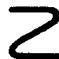
\includegraphics[keepaspectratio]{images/part001_0d60a61e.jpg}}

The definition of Krull dimension is therefore devoid of interest for separated spaces, but it is especially well suited to the topological spaces encountered in Commutative Algebra (spectra of rings, *schemes*, \ldots). In this chapter, no confusion is to be feared with other notions of dimension for topological spaces (for example, that of Lebesgue), and we will simply say “dimension” for “Krull dimension.”

PROPOSITION 1. --- Let X be a topological space.

\begin{enumerate}
\def\labelenumi{\alph{enumi})}
\item
  If Y is a subspace of X, we have \(\dim(\mathbf{Y}) \leqslant \dim(\mathbf{X})\) , and \(\dim_y(\mathbf{Y}) \leqslant \dim_y(\mathbf{X})\) for every point \(y\) of Y.
\item
  Let \(x\) be a point of \(X\) and \(V\) a neighborhood of \(x\) in \(X\) . We have \(\dim_x(X) = \dim_x(V)\) .
\item
  Let \((\mathbf{X}_i)_{i\in I}\) be a finite family of closed subsets of X such that \(\mathbf{X} = \bigcup_{i\in I}\mathbf{X}_i\) . We have
\end{enumerate}

\(\dim(X) = \sup_{i \in I} \dim(X_i)\)and, for every point \(x\) of \(X\)\(\dim_x(X) = \sup_{i \in J_x} \dim_x(X_i)\)\(J\)\(i \in J\)\(x \in X\) , one has

where  denotes the set of  such that .\[
\mathrm{J} _ {x}
\]

Let us prove a). If Z is an irreducible closed subset of Y, its closure \(\overline{Z}\) in X is irreducible (II, § 4, no. 1, prop. 2) and one has \(\overline{Z} \cap Y = Z\) . Thus, every chain \(c\) of closed irreducible subsets of Y defines, by passing to the closure in X, a chain of closed irreducible subsets of X, of the same length as \(c\) . The inequality \(\dim(Y) \leqslant \dim(X)\) follows from this. If U is an open subset of X containing a point \(y\) of Y, we therefore have \(\dim(U \cap Y) \leqslant \dim(U)\) , whence \(\dim_y(Y) \leqslant \dim_y(X)\) .

We prove \(b\) . By definition \(\dim_{x}(X) \leqslant \dim_{x}(V)\) , and the opposite inequality follows from \(a\) ).

We prove \(c\) ). Let \(Z_{0} \subset \ldots \subset Z_{n}\) be a chain of irreducible closed subsets of X. We have \(Z_{n} = \bigcup_{i \in I} (Z_{n} \cap X_{i})\) and each of the sets \(Z_{n} \cap X_{i}\) is closed in \(Z_{n}\) ;

since I is finite, \(Z_{n}\) is contained in one of the \(X_{i}\) . Consequently, we have \(\dim(X) \leqslant \sup_{i} \dim(X_{i})\) , whence equality by \(a\) ).

Now let \(x\) be a point of \(X\) and \(n = \sup_{i \in J_x} \dim_x(X_i)\) , where \(J_x\) is as in the statement. We have \(\dim_x(X) \geqslant n\) by \(a\) ), and, to establish the equality, we may assume \(n\) finite. For every \(i \in J_x\) , let \(U_i\) be an open neighborhood of \(x\) in \(X\) such that \(\dim(U_i \cap X_i) \leqslant n\) . Put \(U = (\bigcap_{i \in J_x} U_i) \cap (\bigcap_{i \in I - J_x} \complement X_i)\) ; the set \(U\) is open in \(X\) . Moreover, we have \(\dim(U) = \sup_{i \in J_x} \dim(U \cap X_i) \leqslant n\) by the preceding paragraph, hence \(\dim_x(X) \leqslant n\) .

COROLLARY. --- a) The dimension of the topological space X is the supremum of the dimensions of its irreducible components (II, § 4, no. 1, definition 2).

\begin{enumerate}
\def\labelenumi{\alph{enumi})}
\setcounter{enumi}{1}
\tightlist
\item
  Let \(x\) be a point of \(X\) . We have \(\dim_x(X) \geqslant \sup_i \dim_x(X_i)\) , where \(X_i\) runs through the family
\end{enumerate}
of irreducible components of X that contain x; there is equality if x has a neighborhood V which has only finitely many irreducible components (which is the case for example if V is Noetherian).


The first assertion is immediate since the chains of irreducible closed subsets of X are the chains of irreducible closed subsets of the irreducible components of X (II, § 4, no. 1, prop. 5). The inequality \(\dim_x(X) \geqslant \sup_i \dim_x(X_i)\) follows

from prop. 1, a). Let V be a neighborhood of x which has only finitely many irreducible components, and let \((\mathrm{V}_{j})_{j\in\mathbb{J}}\) be the family of irreducible components of V that contain x. It follows from prop. 1, b) and c) that we have

\[
\dim_ {x} (X) = \dim_ {x} (V) = \sup _ {j \in J} \dim_ {x} (V _ {j});
\]

we conclude by noting that each of the \(V_{j}\) is contained in one of the \(X_{i}, i \in J_{x}\) , and that consequently we have \(\sup_{j \in J} \dim_{x}(V_{j}) \leqslant \sup_{i \in J_{x}} \dim_{x}(X_{i})\) .

PROPOSITION 2. — Let X be a topological space. We have \(\dim(X) = \sup_{x \in X} \dim_x(X)\) .

Indeed, by definition we have \(\dim(X) \geqslant \dim_x(X)\) for every \(x \in X\) . On the other hand, if \(Z_0 \subset \ldots \subset Z_n\) is a chain of irreducible closed subsets of \(X\) , for all \(x \in Z_0\) and every open neighborhood \(U\) of \(x\) , the sets \(Z_0 \cap U, \ldots, Z_n \cap U\) form a chain of irreducible closed subsets of \(U\) (II, § 4, no. 1, prop. 7). We therefore have \(\dim_x(X) \geqslant n\) , whence \(\dim(X) \leqslant \sup_{x \in X} \dim_x(X)\) .

COROLLARY. — If \((\mathrm{X}_{\alpha})_{\alpha\in\mathbf{A}}\) is an open covering, or a locally finite closed covering, of a topological space X, we have

\[
\dim (X) = \sup _ {\alpha \in A} \dim (X _ {\alpha}).
\]

It suffices to show that, for every point \(x\) of \(X\), one has \(\dim_x(X) = \sup_{\alpha \in A_x} \dim_x(X_\alpha)\), where \(A_x\) is the set of \(\alpha \in A\) such that \(x \in X_\alpha\). This is clear in the case of an open covering, and follows from Proposition 1, c), in the case of a locally finite closed covering.

